% !TEX root = C:\Users\Jan\Documents\dev\Risk-Measurement-Framework\masterthesis_tex\masterthesis_main.tex
\section{Evaluation}
\label{sec:evaluation}

A common example to show backdoor attacks is traffic sign detection (\cite{DBLP:journals/corr/abs-2102-10369}, \cite{DBLP:journals/corr/abs-1708-06733}, \cite{DBLP:conf/codaspy/NudingM20}, \cite{DBLP:journals/tdsc/LiXZZZ21}). That makes it easier to find datasets and already finished ML models to make a case study. The following case study uses a traffic sign dataset and show the risk measurement with the RMF.

\subsection{Evaluation of the ISO 27004 standard in context to the RMF}

After mapping the ISO 27004 to the RMF one result is that this standard should be mapped to a framework if the process stands in relation to a organization and an implemented ISMS.

\subsection{Case Study: Developing a SVM for traffic sign detection}

For the case study scikit-learn \cite{scikit-learn} and for preparation of the dataset in Python OpenCV2 have different function to load and resize images \cite{opencv_library}. In their work, Stallkamp et al. \cite{DBLP:conf/ijcnn/StallkampSSI11} built a mulit-category classification dataset. The mulit-category classification dataset contains german traffic signs for image classification. That mulit-category classification dataset uses the german traffic signs from a approx. 10 hours daytime video from different roads.
This case study is an example to show the functions and results of the RMF. After showing this case study there will be explain and discuss realistic case studies where backdoor attacks could have a more realistic impact for scores of ML models.

\subsection{Preprocessing the original training data}

The original dataset from Stallkamp et al. is splitted between a training and testing folder. The training folder separate 43 signs into subfolders. This subfolders make it easy to use specific traffic signs which decrease the training time. The information of the folders are written in an eponymous csv-file that are not needed further in this case study. In Figure \ref{fig:traffic_signs} the shown traffic signs can be used for training the SVM and are all labeled in the data preprocessing like the subfolder name 0 - 42.

\begin{figure}[h!]
  \centering
  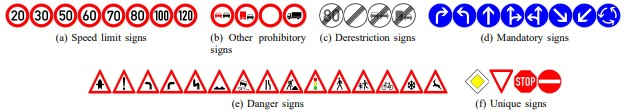
\includegraphics[width=12cm]{pictures/traffic_signs.jpg}
  \caption{Labeled traffic signs adapted from \cite{DBLP:conf/ijcnn/StallkampSSI11}}
  \label{fig:traffic_signs}
\end{figure}

\begin{figure}[h!]
  \centering
  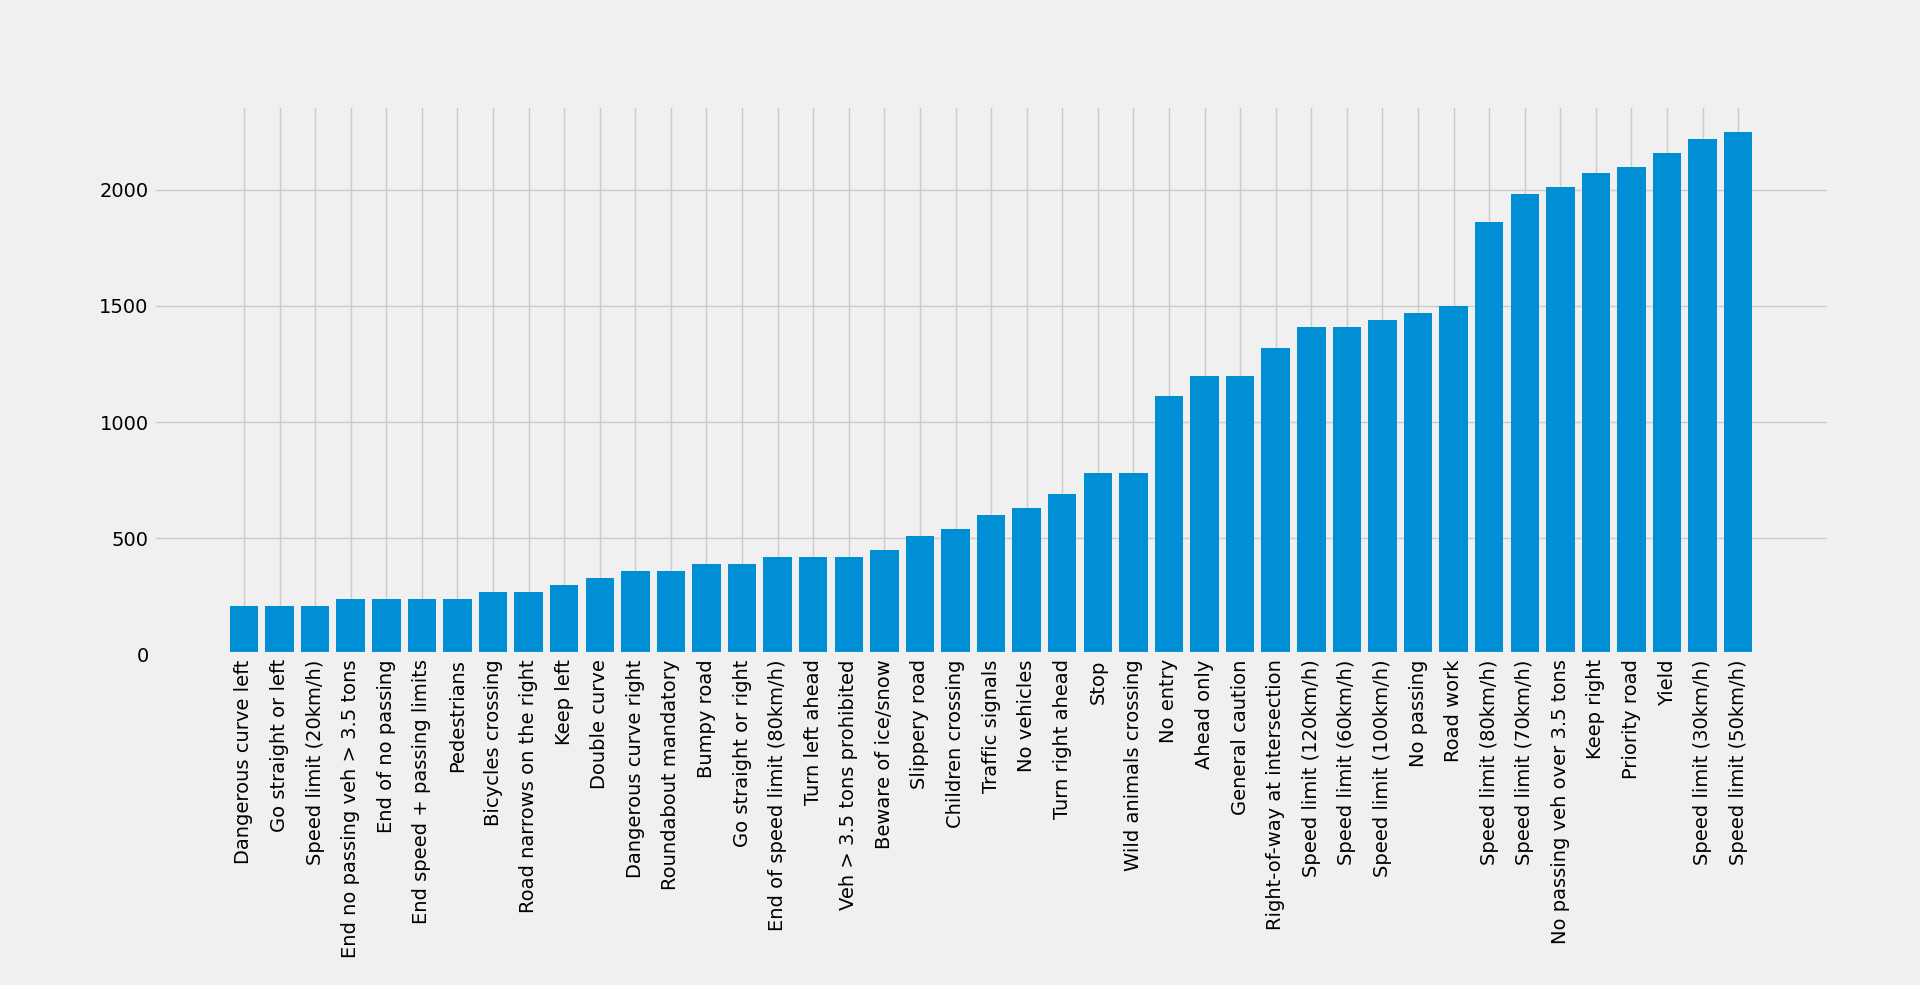
\includegraphics[width=14cm]{pictures/num_of_images.png}
  \caption{Number of images per labels}
  \label{fig:num_of_images}
\end{figure}

All signs are resized to 30x30 pixel and are flattened for the SVM. The training sets are also scaled with the scikit-learn \textit{StandardScaler()} to increase the performance of the training time. The training data are splitted into training and validation data. The test data are an own folder and read in after the training. All functions, the arguments and a description of them can be found in appendix \ref{sec:case_study_functions}.

\subsection{Differences between manipulated and original dataset}

The Python plots from the case study show here based on different ML metrics the differences between the original and manipulated dataset.

\subsection{Results from the risk measurement based on the risk indicators}

\subsection{Poisoning and backdoor attacks in real applications}

Beside the exemplary application from the case study, the scientific papers in this subsection show real applications where the RMF can then help in a more real environment. An example for real-world poisoning attacks against ML models is Microsoft's chatbot Tay. This chatbot learned racist and offensive language from Twitter users \cite{DBLP:conf/iciot/BaracaldoCLSZ18}, \cite{DBLP:conf/ccs/BaracaldoCLS17}. Microsoft removed the bot after 16 hours because the bot produced offensive tweets.

\newpage

\begin{table}[h!]
\begin{minipage}{.5\linewidth}
  \centering
  \begin{tabular}{| l | l | l | l | l |}
  \hline
  \rowcolor{lightgray} Label & precision & recall & f1-score  \\ [0.5ex]
   \hline
   0   &    0.25   &   0.37  &    0.30 \\
   \hline
   1   &    0.71   &   0.86  &    0.78 \\
   \hline
   2   &    0.74   &   0.89  &    0.81 \\
   \hline
   3   &    0.69   &   0.76  &    0.73 \\
   \hline
   4   &    0.87   &   0.76  &    0.81 \\
   \hline
   5   &    0.73   &   0.81  &    0.77 \\
   \hline
   6   &    0.70   &   0.49  &    0.58 \\
   \hline
   7   &    0.89   &   0.77  &    0.83 \\
   \hline
   8   &    0.89   &   0.82  &    0.85 \\
   \hline
   9   &    0.93   &   0.87  &    0.90 \\
   \hline
  10   &    0.94   &   0.91  &    0.93 \\
  \hline
  11   &    0.87   &   0.91  &    0.89 \\
  \hline
  12   &    0.98   &   0.87  &    0.92 \\
  \hline
  13   &    0.95   &   0.98  &    0.96 \\
  \hline
  14   &    0.95   &   0.93  &    0.94 \\
  \hline
  15   &    0.77   &   0.81  &    0.79 \\
  \hline
  16   &    0.74   &   0.97  &    0.84 \\
  \hline
  17   &    0.99   &   0.71  &    0.82 \\
  \hline
  18   &    0.81   &   0.62  &    0.70 \\
  \hline
  19   &    0.39   &   0.53  &    0.45 \\
  \hline
 \end{tabular}
 \end{minipage}%
\begin{minipage}{.5\linewidth}
\centering
  \begin{tabular}{| l | l | l | l | l |}
   \hline
   \rowcolor{lightgray} Label & precision & recall & f1-score \\ [0.5ex]
   20   &    0.53   &   0.59  &    0.56 \\
   \hline
   21   &    0.51   &   0.57  &    0.54 \\
   \hline
   22   &    0.89   &   0.87  &    0.88 \\
   \hline
   23   &    0.48   &   0.49  &    0.49 \\
   \hline
   24   &    0.36   &   0.43  &    0.39 \\
   \hline
   25   &    0.85   &   0.81  &    0.83 \\
   \hline
   26   &    0.80   &   0.80  &    0.80 \\
   \hline
   27   &    0.48   &   0.50  &    0.49 \\
   \hline
   28   &    0.87   &   0.47  &    0.61 \\
   \hline
   29   &    0.52   &   0.91  &    0.66 \\
   \hline
   30   &    0.65   &   0.41  &    0.51 \\
   \hline
   31   &    0.81   &   0.84  &    0.83 \\
   \hline
   32   &    0.37   &   0.60  &    0.46 \\
   \hline
   33   &    0.88   &   0.90  &    0.89 \\
   \hline
   34   &    0.80   &   0.97  &    0.88 \\
   \hline
   35   &    0.89   &   0.84  &    0.87 \\
   \hline
   36   &    0.91   &   0.93  &    0.92 \\
   \hline
   37   &    0.96   &   0.75  &    0.84 \\
   \hline
   38   &    0.96   &   0.88  &    0.92 \\
   \hline
   39   &    1.00   &   0.67  &    0.80 \\
   \hline
   40   &    0.69   &   0.64  &    0.67 \\
   \hline
   41   &    0.40   &   0.73  &    0.52 \\
   \hline
   42   &    0.57   &   0.64  &    0.60 \\
   \hline
  \end{tabular}
  \end{minipage}
\caption{Classification report of the case study}
\label{tab:original_report_1}
\end{table}
